\documentclass[a4paper,10pt,twocolumn]{article}
\usepackage[utf8]{inputenc}
\usepackage{graphicx}
\usepackage{setspace}
\usepackage{caption}
\usepackage{amsmath}
\setstretch{1.2}

%opening
\title{Embeded silicon crystals: Calculating properties from Raman Spectra}
\author{David Omar Flores Tavira}

\begin{document}

\twocolumn[
  \begin{@twocolumnfalse}
    \maketitle
    \begin{abstract}
    In this document we explore the characterization by means of Raman spectroscopy of a silicon layer with a variation of the crystal size.
    Several measurements where made to the system resulting in a set of Raman spectrums that can be analyzed independently. Because the
    desired behaviour of a future algorithm is to threat this as a set itself we propose a class to manage this data and perform operations on this
    spectrums; denoise process with Stavynsk-Golay, Baseline correction and multi peak fitting.
    \end{abstract}
    \vspace{1cm}
  \end{@twocolumnfalse}
]

\section{Introduction}
The system that we are going to analyze is a layer that contains several nano spheres of silicon crystals, The arrangement consists of this stick

\begin{figure}
  \centering
  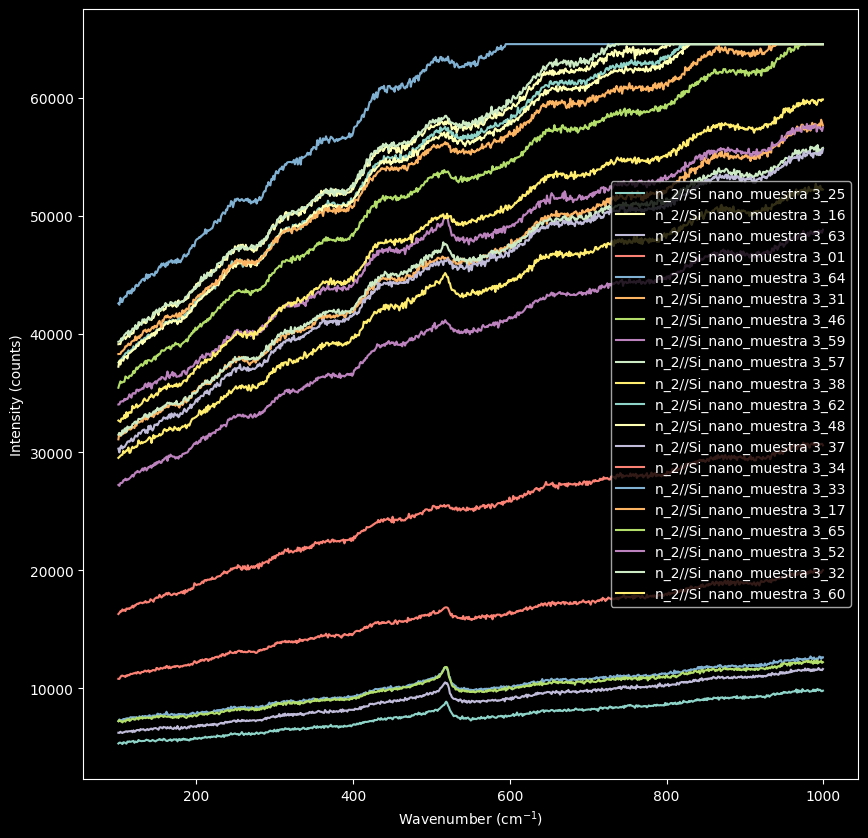
\includegraphics[width=0.9\columnwidth, height=8cm]{all.png}
  \captionof{figure}{Description of the figure.} % Add a caption to the figure
\end{figure}

\section{GPT Architecture}
GPT is built upon the transformer architecture, which has shown exceptional performance in various sequence-to-sequence tasks. We present a detailed overview of the transformer and its key components, including self-attention mechanisms and positional encodings. We then discuss how GPT adapts the transformer architecture for language generation tasks, highlighting the modifications made to enable autoregressive text generation.

    \begin{equation}
    \text{{curve\_fit}}(f, xdata, ydata, p0) \to \text{{popt}}, \text{{pcov}}
    \end{equation}


\section{Training GPT}
The training process of GPT involves pre-training on large corpora and subsequent fine-tuning on specific downstream tasks. We describe the pre-training phase, which involves predicting masked tokens in a language modeling objective. We discuss the challenges and considerations in training GPT on massive datasets, as well as techniques to enhance its performance and efficiency. Furthermore, we delve into the fine-tuning process, where GPT is adapted to specific tasks through supervised learning.

\section{Applications of GPT}
GPT has demonstrated remarkable versatility across a wide array of NLP applications. We provide an overview of the various tasks where GPT has excelled, such as language translation, text summarization, question answering, and sentiment analysis. For each task, we discuss the methodologies employed and the corresponding performance of GPT. We also examine the ethical implications and potential biases that arise when using GPT in real-world applications.

\section{Strengths and Limitations}
While GPT has achieved impressive results, it also exhibits certain limitations. We analyze the strengths and weaknesses of GPT in different contexts, including long-range dependency modeling, handling rare or out-of-distribution words, and dealing with biased or harmful content. We highlight the challenges that researchers and practitioners face when working with GPT and propose potential avenues for improvement.

\section{Conclusion}
In this paper, we have presented a comprehensive analysis of GPT, examining its architecture, training process, and applications. GPT has significantly advanced the field of NLP, demonstrating its capabilities in generating coherent and contextually appropriate text. However, challenges remain in mitigating biases, improving long-range dependency modeling, and addressing ethical concerns. As the field progresses, further research and innovation will pave the way for the continued advancement and responsible use of GPT in diverse real-world applications.

\end{document}
